% !TEX encoding = UTF-8 Unicode
\documentclass[a4paper, titlepage, portuguese]{article}
\usepackage[margin=2.5cm]{geometry}
%\usepackage{fontspec} % XeLaTeX
\usepackage[T1]{fontenc} % LaTeX
\usepackage[utf8]{inputenc} % LaTeX
%\usepackage{newtxmath, newtxtext}
\usepackage{csquotes}
\usepackage{babel}
%\usepackage[backend=bibtex]{biblatex}
%\usepackage[backend=biber]{biblatex}
%\addbibresource{bibliography.bib}

\usepackage{indentfirst}
\usepackage{graphicx}
	\graphicspath{{images/}}
\usepackage{grffile}
\usepackage{float}
\usepackage{amsmath}
	\allowdisplaybreaks
\usepackage{physics}
\usepackage{siunitx}
	\sisetup{inter-unit-product =\ensuremath{.}, output-complex-root=\ensuremath{j},
		complex-root-position=before-number}
\usepackage{hyperref}

% Section styles
%\renewcommand{\thesection}{\Roman{section}}
%\renewcommand{\thesubsection}{\alph{subsection})}
%\renewcommand{\thesubsubsection}{\roman{subsubsection}.}
\renewcommand{\thesubsubsection}{\alph{subsubsection})}

%\titleformat*{\section}{\bfseries\vspace{12pt}\fontsize{14}{6}\rmfamily}
%\titleformat*{\subsection}{\bfseries\vspace{12pt}\fontsize{14}{6}\rmfamily}

% Useful commands
\newcommand{\eq}{\Leftrightarrow} % Equivalente
% Para numerar apenas uma equação
\newcommand\numberthis{\addtocounter{equation}{1}\tag{\theequation}}

% Header and footer
\usepackage{fancyhdr}
\pagestyle{fancy}
\fancyhf{}
\lhead{Electrotecnia Teórica}
\rhead{4º Laboratório}
\lfoot{IST - MEEC}
\rfoot{Página \thepage}
\renewcommand{\headrulewidth}{1pt}
\renewcommand{\footrulewidth}{0.5pt}

% Document
\begin{document}
	\begin{titlepage}
		\center
		\textsc{\bfseries\LARGE Instituto Superior Técnico}\\[1cm] % Name of your university/college
		
\includegraphics[height=1.5cm]{IST_Logo.pdf}\\[2.5cm]

		\textsc{\large Engenharia Eletrotécnica e de Computadores}\\[0.5cm] % Major heading such as course name
		\textsc{\Large Eletrotecnia Teórica}\\[0.5cm] % Minor heading such as course title
		\textsc{\large 2017/2018 2º Semestre}\\[2cm]

		\rule{\textwidth}{1.6pt}\vspace*{-\baselineskip}\vspace*{2pt} % Thick horizontal line
		\rule{\textwidth}{0.4pt}\\[\baselineskip] % Thin horizontal line
			\textsc{\Huge \bfseries 4º Trabalho Laboratorial}\\[0.2cm]
			\bigskip
			\textsc{\large \bfseries Regimes Transitórios}\\[0.2cm]
		\rule{\textwidth}{0.4pt}\vspace*{-\baselineskip}\vspace{3.2pt} % Thin horizontal line
		\rule{\textwidth}{1.6pt}\\[6cm]

		\begin{minipage}{0.9\textwidth}
			\begin{flushleft} \large
				\begin{Large}\bfseries\textsc{Autores}\end{Large}\\[0.4cm]
				\begin{tabular}{l l l}
					Ricardo Simões	& 70389 & \normalsize ricardo.f.d.simoes@ist.utl.pt \\
					Rita Ramos			& 81616 & \normalsize rita.ramos@tecnico.ulisboa.pt \\
					João Pinheiro		& 84086 & \normalsize joao.castro.pinheiro@tecnico.ulisboa.pt \\
					João Sebastião	& 84087 & \normalsize joaofpsebastiao@tecnico.ulisboa.pt \\
				\end{tabular}
			\end{flushleft}
		\end{minipage}\\[0.5cm]

		\large \bfseries Laboratório segunda-feira, 09h30-11h30, Grupo D\\
		\large 14 de maio de 2018\\[1cm]
		\setcounter{page}{0}
	\end{titlepage}

	%\tableofcontents \newpage

	\section{Dimensionamento}
	\subsection{}
		%\begin{figure}[h]
		%	\centering
		%	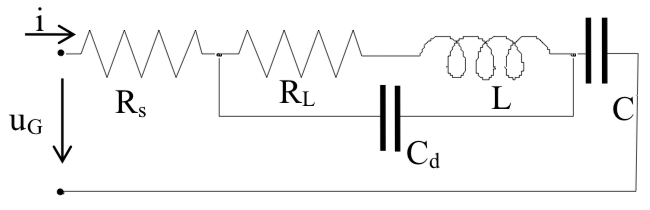
\includegraphics[width=0.6\linewidth]{circuito2.png}
		%	\caption{Circuito RLC tendo em conta a resistência e capacidade distribuídas na bobina}
		%	\label{fig:circuito2}
		%\end{figure}

	%Ver \autoref{fig:figure-example}

	%\printbibliography

\end{document}
